\documentclass[conference]{IEEEtran}
\usepackage{cite}
\usepackage{amsmath, amssymb}
\usepackage{graphicx}
\usepackage{booktabs}
\usepackage{url}
\usepackage{balance}
\graphicspath{{figures/}}
\begin{document}
\title{Bounded Route-Informed Loss Detection in a LEO TCP Model}
\author{\IEEEauthorblockN{Seongchan Kim, Jeongmin Kim, Jaehwan Kang}
\IEEEauthorblockA{Team 5, CS30401 Introduction to Computer Networks\\Fall 2026}}
\maketitle

\begin{abstract}
Forwarding changes in a low Earth orbit (LEO) network can reorder TCP
segments without losing them. We study the supplied ns-3.48
CUBIC/SACK/PRR stack and briefly defer presumed loss only for outstanding
original data associated with a forecast path shortening. The default
loss threshold remains three; a shared deadline and ordinary recovery
evidence limit each episode. At the verified 26.2-second event,
retransmissions fall from three to zero and recovery entries from one to
zero, while whole 200-second goodput increases only 0.02256\%.
A matched genuine loss incurs 5.735961 ms additional first-retransmission
delay. A restricted one-segment tail allowance reduces a 20-MSS
counterexample's completion time from 350.4824 to 257.2237 ms, versus
251.5099 ms for stock TCP. Direct queue observations and a delayed-routing
control show that a later overflow does not require the 75-second
transition. Known-capacity pacing removes bulk queue losses but harms
finite completion. We report this benefit--cost envelope rather than a
universal LEO TCP improvement.
\end{abstract}
\begin{IEEEkeywords}
LEO networks, CUBIC, SACK, reordering, loss detection, finite transfers
\end{IEEEkeywords}

\section{Introduction}
Satellite motion changes forwarding paths even when a LEO network
retains connectivity. A later segment taking a shorter path may arrive
before an earlier segment still in flight. An endpoint that interprets
the resulting acknowledgment evidence as loss can retransmit delivered
data and reduce its congestion window unnecessarily. Hypatia provides a
packet-level framework for examining such route-dependent TCP
behavior~\cite{hypatia}. This question is distinct from recovering a
radio outage: the course model has instantaneous forwarding updates,
fixed capacities and no added random channel loss.

We ask whether accurate advance route information can reduce one
verified unnecessary recovery while bounding exposure to genuine loss.
Our contribution is a small sender modification and an explicit
evaluation of its costs. We retain CUBIC's congestion-control equation,
SACK accounting, proportional rate reduction (PRR), and the retransmission
timeout (RTO). A forecast identifies a limited outstanding sequence
cohort; it does not identify whether those segments will actually be
lost. We subsequently address a finite-transfer cost with at most one
additional final segment. Finally, we diagnose a later queue failure and
evaluate an existing pacing option under known capacity.

The ambiguity is established prior art. TCP Non-Congestion Robustness
(NCR) delays recovery and uses Extended Limited Transmit to preserve
feedback while distinguishing reordering from loss~\cite{ncr}.
RACK-TLP uses transmission-time evidence and probes~\cite{rack}.
Our prototype is neither a complete NCR nor RACK-TLP implementation.
Its particular contribution is forecast-scoped eligibility, bounded
release and measured interactions in the supplied stack. CUBIC is a
standardized controller~\cite{cubic}, but these results do not establish
superiority over current Linux TCP or BBR.

\section{Problem Statement}
\subsection{Presumed loss during a forwarding change}
The supplied Seoul--London state contains a path-shortening event at
26.2 s. In the baseline trace, a SACK block above outstanding holes meets
the stock presumed-loss rule and causes three retransmissions within one
recovery episode. Transmission identities, positive receiver acceptance,
application delivery and subsequent cumulative acknowledgment establish
that the originals were delivered. Connected drop hooks show no matching
drop for those originals. Geometry or a window decrease alone would not
establish unnecessary recovery, and three retransmissions must not be
reported as three recovery entries.

This stack infers loss using duplicate-ACK and SACK packet-count evidence.
The relevant first episode is not adequately described as simply three
consecutive duplicate ACKs: SACK marking can classify several holes
before the head is processed. Protecting only the head therefore leaves
other members of the same old-flight cohort marked lost. A useful
intervention must consistently handle eligible holes while preserving
the evidence for unrelated losses.

\subsection{Loss delay and insufficient finite feedback}
Additional reordering tolerance can delay a real retransmission.
Moreover, the time spent waiting is not an upper bound on transfer
completion cost. In a stable 20-MSS transfer with its first segment
physically dropped and an intentionally wrong shortening hint, a
6.631518 ms deferral changes ACK/PRR timing. The final unsent segment then
waits approximately another round. All 27,600 B still arrive, so
bytes divided by the complete 4-second observation would hide the
completion penalty. PRR deliberately controls transmission during
recovery~\cite{prr}; its accounting must not be replaced with fictitious
delivery or a reduced pipe estimate.

Avoiding an earlier window reduction can also change later queue
history. Around 75 s, the selective trace carries a larger source queue
before the routing update. It is tempting to attribute subsequent drops
directly to path shortening and cap the window by geometric BDP. That
causal claim requires direct queue and routing controls: smoothed RTT
does not separate queue residence from propagation, and a geometric
window cap can discard useful queue headroom.

\section{Proposed Ideas}
\subsection{A forecast-scoped, shared loss deadline}
Let a supplied forecast describe a forward transition at time $T$,
old/new forward propagation delays $d_o, d_n$, and corresponding
propagation RTTs $R_o, R_n$. We select transitions whose forward path
changes and $d_o-d_n\ge 1$ ms. Two events, 26.2 and 75 s, satisfy this rule.
The sender registers outstanding originals transmitted no later than $T$.
Registration expires after
\begin{equation}
 H=2\max(R_o, R_n).
\end{equation}
Membership is based on outstanding sequence/transmission history, not
knowledge of the packet's remaining physical path.

When ordinary SACK marking first suspects an eligible hole, one episode
deadline is created using
\begin{equation}
 \tau=\operatorname{clamp}\bigl(2(d_o-d_n), 1\mathrm{ms}, 20\mathrm{ms}\bigr).
\end{equation}
The effective deadline never exceeds registration expiry. Other eligible
holes share it; later SACKs or a new head do not extend it. A predeclared
SACK-size budget is
\begin{equation}
 B=3+\left\lceil\frac{r(d_o-d_n)}{8 M}\right\rceil,
\end{equation}
where $r$ is the configured link rate and $M$ is the MSS. This is a
conservative experimental rule, not a proved overtaking bound: queues,
bursts and reverse-path ACKs are not determined by geometry.

The default loss threshold remains $K=3$. The stock SACK loss inference is
based on packet evidence~\cite{sack}. SACK and delivered-byte
accounting continue during the deferral. Covering acknowledgment, expiry,
budget excess, stock marking outside the cohort, ECN, existing recovery
or RTO release protection as applicable. The implementation does not
erase already marked losses. Expiry reevaluates stored evidence and
wakes ordinary recovery without requiring another ACK. An OPEN-state
repair enters recovery only when a native head loss flag exists; that
branch was not exercised in the reported cases and is not claimed as an
executed boundary test. Normal RTO behavior is unchanged.

The forecast is an oracle input from the supplied forwarding plan.
Deployment would require an operator to identify the affected sender and
deliver route/time information before the event. Public orbital elements
alone do not reveal routing policy or queue state. Notice delivery,
clock error, cancellation and prediction error are not implemented.

\subsection{A one-MSS final-segment allowance}
After ordinary ACK/SACK processing and \texttt{SendPendingData} have used
normal transmission allowance, the sender can admit at most one extra
original segment per active deferral episode. Admission requires fresh
unique SACK evidence, application termination intent, exactly 1..MSS
unsent bytes, a new-data frontier equal to the original high-TX frontier,
receiver-window room and
\begin{equation}
 \mathrm{pipe}+\mathrm{newBytes}\le\mathrm{cwnd}+M.
\end{equation}
The original episode deadline remains intact. The hook invokes normal
packet transmission, FIN, callback, rate and retransmission accounting.
It does not increment cwnd, fabricate an ACK, count the same SACK twice
as delivered data, or accelerate the lost segment's deadline. This is a
restricted extra-segment allowance, not ``tail credit'' recovered from
already consumed SACK evidence or an implementation of TLP.

The restriction deliberately refuses two or more remaining segments.
We test 21 MSS as a boundary, rather than widening admission after seeing
its completion time. A 100 GB bulk flow is far from its application tail,
so this addition is expected to remain inactive there.

\subsection{Known-capacity pacing as a conditional companion}
To address observed source backlog, we compare existing native pacing
with the same pacing constrained by a known fixed link rate. Its timer
accounts payload bytes, whereas a full data packet is 1434 B for 1380 B
payload. We retain native pacing behavior~\cite{ns3} and set its ceiling to
\begin{equation}
 r_{\max}=\left\lfloor r_{\mathrm{link}}\frac{1380}{1434}\right\rfloor.
\end{equation}
This gives 9,623,430 bps at 10 Mbps and 96,234,309 bps at 100 Mbps. Native
slow-start/avoidance pacing ratios, initial-window behavior, CUBIC and
loss recovery remain unchanged. Initial bursts and direct retransmissions
remain, so the ceiling is not a strict wire shaper. Known total capacity
does not reveal a competing flow's available share. Pacing is evaluated
as an established conditional option, not the forecast policy's novelty.

\section{Experiment Setup}
\subsection{Fixed course model and controls}
We use the official pinned Docker image and its ns-3.48/Hypatia source.
The provided Seoul 1584--London 1585 state updates forwarding every 100 ms.
Satellite geometry continues to evolve; forwarding changes instantly.
We add no handover outage, varying link capacity, random radio error or
new topology. Bulk runs use CUBIC/SACK/PRR, 1380 B MSS, initial cwnd 10 MSS,
one 100 GB flow starting at 0 s, 10 Mbps links, 100-packet device queues,
seed 123456789 and 200 s duration. The bulk file is incomplete at 200 s;
its metric is ordered application goodput, not file completion time.

\begin{table}[t]
\caption{Core matched controls and their purpose}
\label{tab:setup}
\centering
\begin{tabular}{p{0.93 in}p{2.20 in}}
\toprule
Family & Fixed comparison\\
\midrule
Natural LEO & Stock, selective, selective+tail; whole 200 s and
first[25.7, 28.2)s.\\
Actual old-flight loss & Physically drop one matching original during
shortening; stock/selective+tail.\\
Finite loss & Stable 100 Mbps, 50 ms one-way, q 2000, 4 s; first-segment
loss, wrong hint, 20 MSS; stock/selective/tail.\\
Admission boundary &21 MSS selective/tail; two remaining segments must
not bypass ordinary allowance.\\
Queue causality & Natural stock/selective observers; fixed selective
policy with the 75 s routing delta delayed to 78 s.\\
Pacing & OFF/native/known-capacity bulk; selected pacing then tested
with first-original loss and finite 20 MSS.\\
\bottomrule
\end{tabular}
\end{table}

The injected old-flight LEO pair drops the same original at the same
receiver time, verified by flow/TX ID/TX time/sequence/payload. The
finite control intentionally gives an incorrect positive hint on a
stable path; ignoring that hint using knowledge of actual loss would
conceal the safety cost. Additional pacing loss controls use a fixed
first-original-segment rule and record actual identities per arm.

\subsection{Measurements and reproducibility}
Application goodput is unique ordered receiver bytes times eight divided
by the exact interval. Finite FCT requires every expected byte and is
measured from the declared flow start to last application delivery.
RETX events and recovery-state entries are distinct counters. Full
transmission tags identify original acceptance and drops; packet UID
alone is insufficient because fragments/bursts can reuse it. Wire receive
traces precede TCP processing and are not substituted for application
delivery.

Passive hooks identify native device queues, exact packet enqueue and
serialization start, stop/wake flags, and the no-root stopped-device
TrafficControl rejection. Queue occupancy is integrated from actual
state transitions, not flush snapshots or SRTT. Source waiting and
downstream queues are measured separately. Drop/pending residence is
censored separately from successfully served residence. All-layer losses
are deduplicated tagged payload-bearing transmissions; ACK/control or
unmapped notifications are separately reported.

Each declared condition is one deterministic run, not a statistical
replicate. Launch/package identities, commands and environment are
recorded; source patches, configuration, forecast/state,
binary/libraries and outputs are hashed. An extracted Git-free package
records source-file identity rather than inventing a launch commit.
Instrumentation-OFF/observer controls reproduce historical measurement
CSVs; immutable runtime and queue conservation are checked before
interpretation. Three backpressure outcome files have a narrowly verified
exception: ordered non-pending rows match, while pointer-ordered final
pending rows match as full-field multisets. Original raw hashes remain
recorded; no other measurement comparison is relaxed.
Fresh-package replay receipts are reported separately
from historical archive/member verification. Neither a successful build
nor an unexercised source branch is an executed safety proof.

\section{Evaluation}
\subsection{An event-local benefit and a small whole-run gain}
Figure~\ref{fig:event} shows the actual window trajectory around the event.
At the verified 26.2 s episode, selective protection waits
26.328788841--26.334460816 s, 5.671975 ms, and covering acknowledgment
releases it before the 6.631518 ms maximum for that hint. The first window
has 3 RETX/1 recovery for stock and 0/0 for selective. Ordered goodput
improves from 9.485568 to 9.622464 Mbps, 1.443203\%.

\begin{figure}[t]
\centering
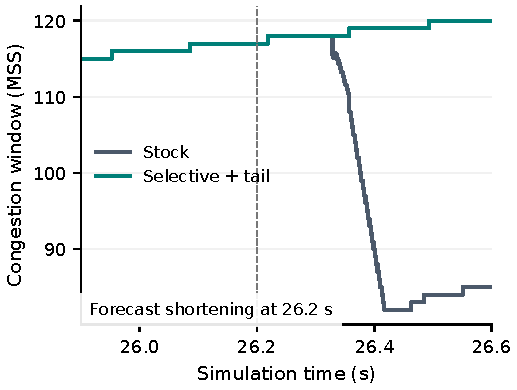
\includegraphics[width=\columnwidth]{natural-event.pdf}
\caption{Actual congestion-window steps around the 26.2 s shortening.
Selective+tail avoids the stock recovery reduction; tail admission is
inactive in bulk. The whole-run goodput gain is only 0.02256\%.}
\label{fig:event}
\end{figure}

Across 200 s, stock delivers 238,608,900 B at 9.544356 Mbps, versus
238,662,720 B at 9.5465088 Mbps for selective:53,820 B, or 0.022556\%.
Whole RETX/recovery changes 523/41 to 507/40. This entire difference is
not independently classified as spurious retransmission removal. Tail
admission occurs zero times in the 100 GB flow and its trajectory matches
selective, so the bulk gain must not be credited to the tail allowance.
The later[74.5, 77.0)s window is worse for selective:12 RETX/2 recoveries
versus 0/0, with no active selective wait there. Earlier intervention has
changed subsequent history; this is not a direct effect of a new 75 s wait.

\subsection{Genuine-loss cost and finite-tail repair}
In the matched old-flight LEO pair, physical loss to first RETX is
49.468699 ms for stock and 55.204660 ms with selective/tail, a 5.735961 ms
extra delay. This is one verified matching loss, not an end-to-end
recovery-time bound. Budget excess releases protection before its timer;
both arms have 500 tagged data losses over the run and almost identical
bulk delivery.

Figure~\ref{fig:finite} shows the finite counterexample. Stock completes
27,600 B in 251.509920 ms; selective takes 350.482400 ms, despite waiting
only 6.631518 ms longer for the first RETX. Tail admission sends the
last original 1380 B segment at 0.201165760 s. Completion becomes
257.223678 ms:93.258722 ms earlier than selective, still 5.713758 ms later
than stock. The wait and first RETX time are unchanged. All three arms
have one real loss, one retransmission and one recovery.

\begin{figure}[t]
\centering
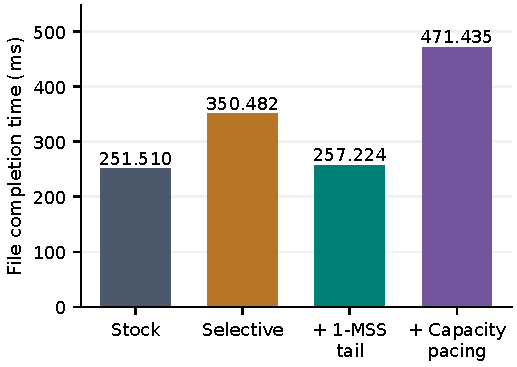
\includegraphics[width=\columnwidth]{finite-cost.pdf}
\caption{Completed 20-MSS transfers with a real first loss and wrong
forecast. One-MSS admission repairs most selective cost; bulk-selected
pacing reintroduces a substantial finite cost.}
\label{fig:finite}
\end{figure}

At admission, cwnd remains 13,800 B while allowed pipe reaches at most
15,180 B. This explicit 1 MSS exception is not free recovered credit.
The 21-MSS boundary has zero admissions and identical 350.597120 ms FCT
for selective and tail. The same tail restriction is inactive in bulk
and in the injected bulk-loss pair. Added-segment loss, a blocked
receiver window, FIN at the receiver-window boundary and all ECN/RTO
orderings are not covered by these experiments.

\subsection{What the 75-second routing control establishes}
Direct source measurements locate the failure at Seoul device 1/txq 0:
a 100-packet DropTail queue, no root qdisc and no QueueLimits. At 100
queued packets the device-stop flag is set; incoming packets are then
rejected in TrafficControl's no-root branch. This is distinct from a
DropTail enqueue failure. Selective already has mean 71.1786 queued
packets in[74.5, 75)s versus stock 43.3501. The post[75, 75.5)s means
are 87.2324 versus 53.2709, with actual served waits 96.1995 versus
59.6231 ms and 100\% source serialization utilization.

To test necessity of the 75 s transition, we move precisely its 30 sparse
forwarding rows to 78 s, leave later overrides intact and retain the
original forecast/policy schedule. Accumulated forward/reverse paths and
native interfaces are checked at every affected 100 ms frame. Packet,
window and projected observer history before 75 s matches exactly.
This changes two-direction routing/link choices under the ideal shared
GSL model, not only propagation delay or a physically verified handover.

The delayed-route arm still fills at 75.617356228 s and first rejects at
75.644889535 s, before 78 s. It retains 11 focus drops and 12 RETX/2 recoveries,
although individual drop identities/times differ. Therefore the 75 s
transition is not necessary for this local overflow under fixed prior
policy history. Routing affects timing; this control neither proves it
has no effect nor justifies a universal geometry-only window cap.

\subsection{Pacing benefit has a finite-flow boundary}
Figure~\ref{fig:queues} compares the bulk companion with the unchanged
selective/tail control. Known-capacity pacing passes the prospective
99.5\% goodput-retention gate:9.5465088 to 9.5662704 Mbps. Whole tagged
data losses fall 486 to 0, RETX 507 to 2 and recoveries 40 to 1. Post source
queue/wait is zero for the 436 actually served packet visits. Across the
whole run, source residence mean falls 41.724668 to 0.000456345 ms;
initial burst still peaks at 10 queued packets and downstream queues
remain. Source zero does not mean zero network buffering.
The two residual retransmissions have original-TX/receiver/APP witnesses
proving prior ordered delivery; their cause was not isolated.

\begin{figure}[t]
\centering
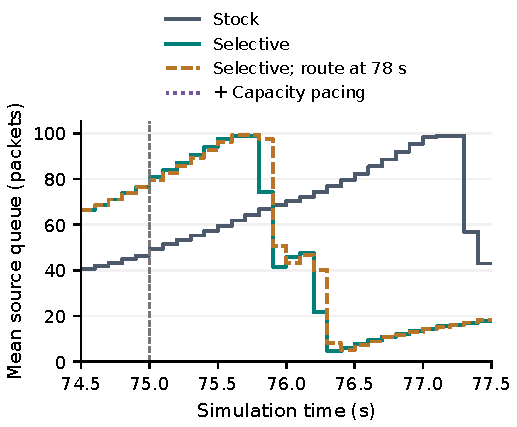
\includegraphics[width=\columnwidth]{queue-causality.pdf}
\caption{Mean source backlog in 100-ms bins over [74.5,77.5) s. Delaying routing does not remove
overflow; a separate known-capacity pacing option lowers bulk backlog.
The intervention changes routing, not geometry alone.}
\label{fig:queues}
\end{figure}

Two standard queue-management controls keep the nominal source queue
budget at 100 packets: FIFO 96 plus device 4, and native-default CoDel 96
plus device 4. FIFO only relocates backlog: combined source residence,
goodput and 486 data losses are unchanged. CoDel, an existing sojourn-time
AQM~\cite{codel}, lowers mean residence to 3.432026 ms and whole losses
to 171, but goodput is 8.9403576 Mbps ($-6.3495\%$). Intentional CoDel
drops count as losses; requeue and in-service slots lie outside nominal
capacity and are separately measured. This comparison does not generally
disprove CoDel; its fixed defaults miss the declared retention gate here.

Native pacing without the capacity ceiling delivers 9.0571056 Mbps,
below the gate. The selected paced arm's first-original-loss bulk
control delivers 9.332664 versus 9.3421584 Mbps for current policy
($-0.1016\%$); the first-loss-to-RETX delay is 53.228969 ms in both.
This initial loss control does not replace a loss during active
forecast protection.

Finite pacing is unfavorable: FCT rises from 257.223678 to 471.434773 ms,
83.28\%. Despite a 96.234309 Mbps ceiling, the native computed rate is
only 2.208 Mbps, yielding 5 ms spacing. Tail checks still see more than
one MSS remaining and make no admission. It is incorrect to attribute
the cost solely to a pacing-timer guard or to claim that merely calling
the tail hook at timer expiry fixes it. We therefore do not make pacing
a global default. No stock-plus-capacity-only arm, competing flows,
varying capacity or parameter sweep establishes its independent or
deployment-wide effect.

\begin{table}[t]
\caption{Effect magnitudes and costs in the matched controls}
\label{tab:magnitudes}
\centering
\begin{tabular}{lrr}
\toprule
\multicolumn{3}{l}{Completed 20-MSS first-loss transfer}\\
Policy & FCT (ms) & Tail TX\\
\midrule
Stock & 251.509920 & 0\\
Selective & 350.482400 & 0\\
Selective + tail & 257.223678 & 1\\
+ Capacity pacing & 471.434773 & 0\\
\midrule
\multicolumn{3}{l}{Natural 200 s bulk; no finite FCT}\\
Policy & Goodput (Mbps) & Data losses\\
\midrule
Stock & 9.5443560 & 499\\
Selective + tail & 9.5465088 & 486\\
+ Capacity pacing & 9.5662704 & 0\\
\bottomrule
\end{tabular}
\end{table}


\balance
\section{Conclusion}
A short, forecast-scoped SACK-loss deferral avoids a verified unnecessary
recovery without globally increasing the default loss threshold. Its
benefit is local and the whole-run gain is small. Genuine-loss and finite
controls expose costs that goodput over a long observation would hide.
One extra final original segment recovers most of the observed finite
cost while retaining the shared deadline and explicit 1 MSS limit.

Direct queue identity, occupancy and routing controls are necessary to
avoid blaming every later loss on geometry. Known-capacity pacing is
useful in the fixed bulk case but substantially worsens the tested short
transfer. The defensible result is a bounded prototype with measured
failure conditions, not universal reordering immunity, a replacement for
modern TCP, or a deployment-ready controller. Competition, uncertain
forecasts, variable links and additional loss/FIN/ECN boundaries remain
future validation.

\begin{thebibliography}{1}
\bibitem{hypatia}
S. Kassing, D. Bhattacherjee, A. B. Aguas, J. E. Saethre, and A. Singla,
``Exploring the `Internet from space' with Hypatia,'' in \emph{Proc. ACM IMC},
2020, pp. 214--229, doi:10.1145/3419394.3423635.
\bibitem{cubic}
L. Xu, S. Ha, I. Rhee, V. Goel, and L. Eggert,
``CUBIC for Fast and Long-Distance Networks,'' RFC 9438, Aug. 2023.
\bibitem{ncr}
S. Bhandarkar, A. L. N. Reddy, M. Allman, and E. Blanton,
``Improving the Robustness of TCP to Non-Congestion Events,'' RFC 4653,
Aug. 2006.
\bibitem{rack}
Y. Cheng, N. Cardwell, N. Dukkipati, and P. Jha,
``The RACK-TLP Loss Detection Algorithm for TCP,'' RFC 8985, Feb. 2021.
\bibitem{prr}
M. Mathis, N. Dukkipati, and Y. Cheng,
``Proportional Rate Reduction for TCP,'' RFC 6937, May 2013.
\bibitem{codel}
K. Nichols, V. Jacobson, A. McGregor, and J. Iyengar,
``Controlled Delay Active Queue Management,'' RFC 8289, Jan. 2018.
\bibitem{sack}
E. Blanton, M. Allman, L. Wang, I. Jarvinen, M. Kojo, and Y. Nishida,
``A Conservative Loss Recovery Algorithm Based on Selective
Acknowledgment (SACK) for TCP,'' RFC 6675, Aug. 2012.
\bibitem{ns3}
ns-3 Project, ``TCP models,'' \emph{ns-3 Model Library},
\url{https://www.nsnam.org/docs/models/html/tcp.html}.
\end{thebibliography}
\end{document}
